
%\documentclass[twocolumn,letterpaper]{article}
\documentclass[10pt]{csce}

\usepackage[hmargin=.75in,vmargin=1in]{geometry}
\usepackage[american]{babel}
\usepackage[T1]{fontenc}
\usepackage{times}
\usepackage{caption}
\usepackage{flushend}

\usepackage{gensymb,hyperref,graphicx,paralist,amsmath,multirow}
\usepackage[table]{xcolor}
\pagenumbering{gobble}

\title{\bf A Model-Based Scheduling Framework for Enhancing Robustness}

%%%% Make sure the author names are boldface.
\author{
{\bfseries Nicolas Grounds and John K. Antonio}\\
School of Computer Science, University of Oklahoma, Norman, Oklahoma, United States of America\\
}

\begin{document}

\maketitle                        %%%% To set Title and Author names.

\begin{abstract}
In previous work the performance of scheduling algorithms for dynamic
scheduling of tasks in a distributed system were evaluated for their
robustness to error in the model of tasks' information.  There it was
found that incorporating task completion timings from the actual distributed
system into the algorithms' model of the system was crucial for achieving
robustness.  In this paper, various degrees of feedback, rather than simply
all-or-none, are evaluated using the same simulated studies as in previous
work and a proposed strategy for biasing model tasks' information is proposed
in order to counteract the most egregious effects of model error on
performance.
\end{abstract}


\vspace{1em}
\noindent\textbf{Keywords:}
 {\small distributed system, scheduling, performance, robustness, biasing}


\section{Introduction and Background}
\label{sec:Intro}

Scheduling computational tasks to machines so as to improve specified metrics
of performance has been the topic of a plethora of good work produced over the
past several decades \cite{taxonomy}. The underlying assumptions and objectives
of this body of work varies along several dimensions. First, some work assumes
all tasks are independent whereas other work, as in this paper, allows for
tasks to have dependency or precedence relationships with other tasks (for
which interrelated tasks are typically represented in a directed acyclic graph,
or DAG). Additionally, there are static formulations to scheduling in which a
desired schedule is detemined offline based on assumed knowledge related to the
machines' available resources and, correspondingly, the resource requirements
of the computational tasks.

Conversely, this paper addresses dynamic scheduling in which the schedule for
tasks is determined online in real-time with the execution of those tasks on a
distributed system. Unlike the static scheduling problem, dynamic scheduling
does not require upfront knowledge of the arrival of future tasks into the
system for scheduling. Algorithms for dynamic scheduling make use of knowledge
about the tasks which are ready for scheduling and their resource requirements
such as CPU and memory load as well as the resource capacities of the machines
in the distributed system.

Such algorithms for dynamic scheduling may be based on heuristics for selecting
which tasks to prioritize execution of and determining when to begin their
execution and on which machine. Other algorithms may actively attempt to
optimize scheduling decisions with respect to a desired outcome based on a
user-defined objective.  Both types of algorithms are generally measured
and compared to one another against such objectives such as minimizing makespan
(time required for completed execution of all tasks) \cite{stochastic}, or, as
in this paper, the degree to which all tasks of a DAG are completed by a
DAG-associated deadline.

Scheduling algorithms may orthogonally be evaluated based on their robustness,
for example, how well the same objective is achieved when information provided
to the scheduling algorithm contains errors such as inaccuracies in the
amount of resource requirements of the tasks.  In previous work \cite{pdpta18}
four dynamic scheduling algorithms' robustness to error with respect to
performance against an objective of completing DAGs before their deadline was
presented, showing how some algorithms were not robust to even the smallest
amount of simulated error.  Additionally, the use of task completion time
feedback from the actual distributed system back into the modeled system used
by the scheduling algorithms was found to substantially improve robustness of
all four scheduling algorithms to even large amounts of simulated error.

The remainder of the paper is organized in the following manner.  Section
\ref{sec:Framework} describes the problem domain and the simulation software's
use of modeling the distributed system where errors in task requirements may
be inherent.  Section \ref{sec:Biasing} presents an approach to counteracting
model error to prevent scheduling algorithms from over-committing system
resources to executing too many tasks concurrently. Section \ref{sec:Results}
presents results of simulated case studies within that software simulator.
Finally, Section \ref{sec:Summary} summarizes the findings from these
simulations and presents the conclusions of our work.


\section{Problem Domain and Simulation Environment}
\label{sec:Framework}

The present work is an extension to previous work \cite{pdpta18} in which a
model-based approach to dynamically scheduling tasks from DAGs (called
workflows) was introduced.  Four scheduling algorithms were tested in a
simulation environment \cite{soasim} given the same 24-hour simulated period
of arriving workflows ranging in size from 5 tasks up to 800.  Each workflow
had a known, predetermined deadline and scheduling algorithms were evaluated
based both on the number of workflows completed before their deadline and the
distribution of workflow counts completed at various normalized proportions
past their deadline (e.g., workflows up to 100\% late relative to the amount
of time between their arrival and deadline).

Scheduling algorithms are used to determine from a given queue of tasks
ready to begin executing (i.e. tasks of arrived workflows that have no
precedence constraints or whose precedent tasks have all completed) both
when the task should begin executing and on which machine of the platform.
Unlike some scheduling research, tasks are permitted to executing concurrently
with other tasks on the same machine which increases machines' overall load
on resources such as CPU and memory and thereby slows the rate of work on each
executing task.  Original work in \cite{pdpta09} details this non-linear
degradation of rate of work (efficiency) due to concurrent task execution.

Figure \ref{fig:platform} illustrates the various components and general
flow of information within the model-based approach to executing and evaluating
scheduling algorithms.  Whereas the modeled tasks' requirements (CPU load,
required number of CPU cycles, and memory load) may contain errors relative to
the true values of those tasks, the model platform may diverge from the
actual platform in terms of which tasks are completed and which are still
executing.

\begin{figure}
	\begin{center}
		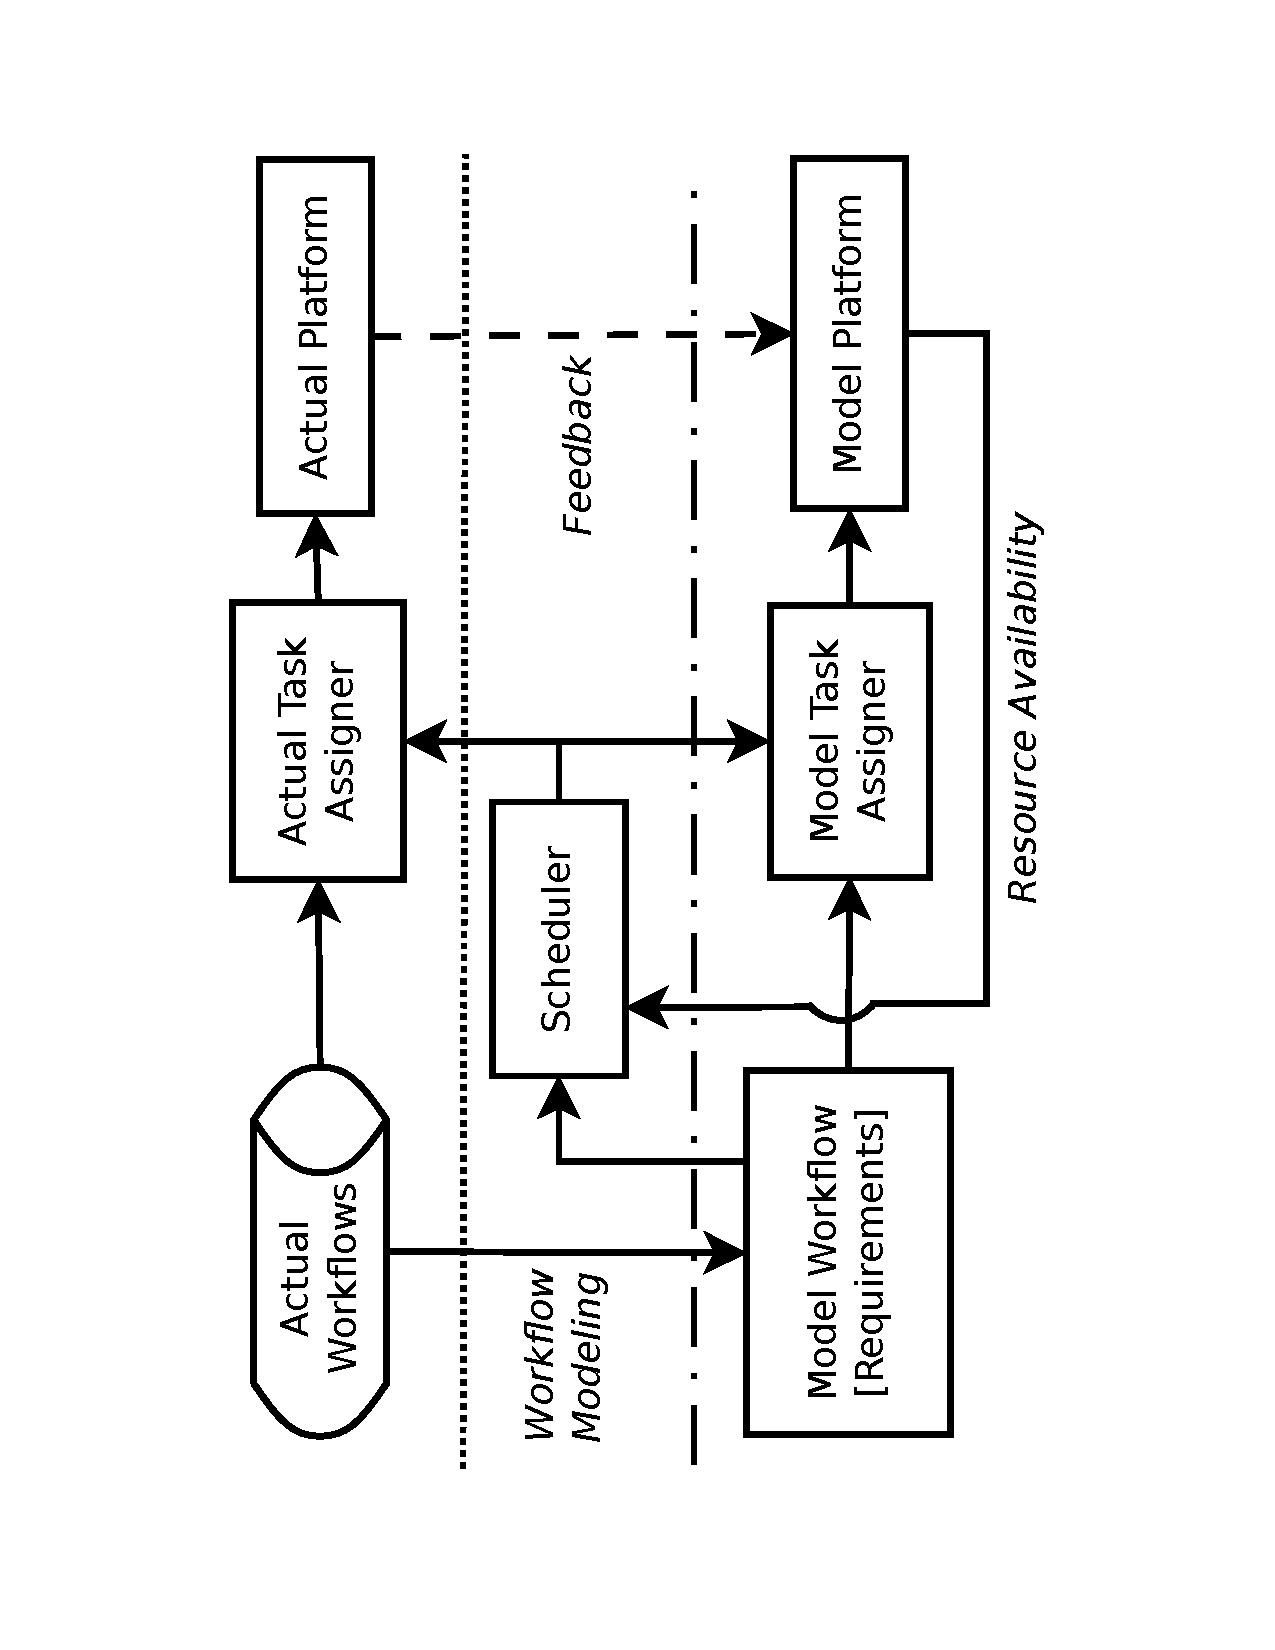
\includegraphics[angle=-90,width=0.5\textwidth]{figures/PlatformDiagram.pdf}
	\end{center}
	\caption{Block diagram illustrating model-based framework from
		\cite{pdpta18}.}
	\label{fig:platform}
\end{figure}

All four studied scheduling algorithms were shown to be sensitive to
even small amounts of error in modeled tasks.  Each scheduling algorithm
exhibited a decreased percent of workflow completed ahead of their deadline
with the smallest amount of error studied.  For three of the scheduling
algorithms the decrease was substantial, but relatively equal, regardless of
the amount of error.  For the fourth scheduling algorithm, the decrease was
less severe overall and was propotionate to the amount of error.  The
fourth algorithm was thus declared to be somewhat robust to small amounts of
error (less than 0.5\%) but ultimately, like all three others, was not
robust for errors of 1\% or greater.

The main result of \cite{pdpta18} showed that incorporating feedback of
task completions from the actual platform to the model platform thereby
preventing the model platform from modeling a task completing before the
actual task completed dramatically increased robustness of all scheduling
algorithms for even errors up to 90\% (the highest amount studied).  Figure
\ref{fig:underestimating} illustrates why the model platform underestimating
the requirements of a task and thereby modeling it as completed ahead of the
actual task can be so detrimental.

\begin{figure}
	\begin{center}
		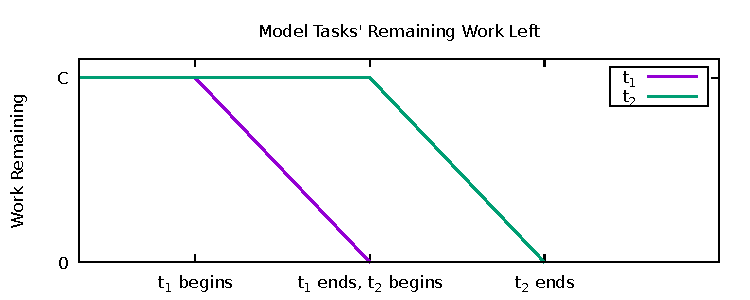
\includegraphics[width=0.5\textwidth]{figures/UnderestimatedErrorEffect_ModelTaskWork.pdf}
		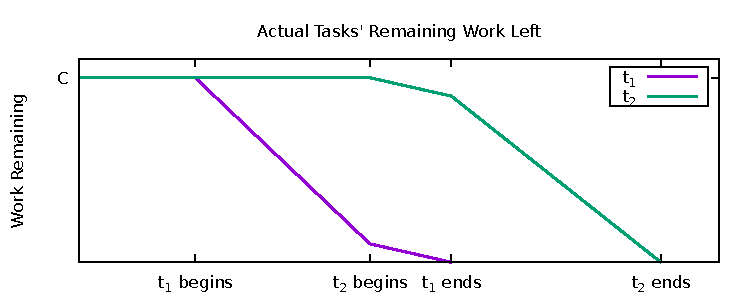
\includegraphics[width=0.5\textwidth]{figures/UnderestimatedErrorEffect_ActualTaskWork.pdf}
	\end{center}
	\caption{Illustrating the disconnect due to error such that model task
		requirements underestimate actual task requirements and the model
		task finishes ahead of the actual task.}
	\label{fig:underestimating}
\end{figure}

In Figure \ref{fig:underestimating} two tasks, $t_1$ and $t_2$, both have
the same amount of CPU cycles, $C$, required for their completion.  In the
top half is the modeled platform's view of time in which task $t_1$ begins
executing first and when it completed, $t_2$ is scheduled to immediately
begin executing.  However, because the modeled requirements of $t_1$ were
an underestimate of the actual $t_1$'s requirements, when the model of
$t_1$ finishes and $t_2$ is scheduled to begin, the actual platform is not
yet finished with $t_1$ and thus must work concurrently on $t_1$ and $t_2$
for some time until the actual $t_1$ task does complete.  This causes both
$t_1$ and $t_2$ to have actual completion times later than the modeled
completion times because of the unintentionally-overallocated resources of
the machine executing the tasks.  By extension, if another task, say $t_3$,
were to be scheduled to begin after $t_2$ finishes this problem could compound
because $t_2$'s actual completion would delayed by concurrent execution with
$t_1$ and further delayed by concurrent execution with $t_3$.

The previous example illustrates why allowing the model to platform to
inform scheduling algorithms when tasks are complete and machines are
idle (or less loaded) in the presense of error which may underestimate tasks'
true requirements can be so detrimental.  With feedback of every task's
completion from the actual platform the modeled completion times of tasks
may be safely ignored.  However, complete feedback of all tasks' completion
may be impractical in a live system, or may simply be cost-prohibitive.
This paper thus seeks to address the question of whether partial feedback
of tasks' completion times may be sufficient to achieve some level of
robustness to model error.  In addition, based specifically on the
knowledge of the underestimating problem illustrated prior, in Section
\ref{sec:Biasing} that follows a specific approach to counteracting
that problem by biasing model task requirements is proposed.  Results of
both partial feedback and biasing are presented in Section \ref{sec:Results}.


\section{Biasing Model Requirements}
\label{sec:Biasing}

As illustrated in Figure \ref{fig:underestimating}, if the model task
requirements are an underestimate of the actual task's requirements then
scheduling algorithms may schedule future tasks to begin executing
unintentionally-concurrent with other tasks, delaying their completion.
However, if the model is known to have error which may underestimate
task requirements, then the model task requirements could simply be
biased by increasing its value in order to reduce (or ideally, eliminate)
the probability that it underestimates the actual task requirements.
In this section three proposed strategies for biasing model task
requirements are proposed.

The simplest form of biasing would be to add a constant value to each
task requirement.  If the maximum magnitude of error for which a model
task requirement may underestimate the actual task requirement is known,
then that value would be the ideal bias constant value because it would
eliminate the model from ever underestimating task requirements but
bound the worst overestimate to the smallest amount possible for such a
constant value biasing strategy.  Practically, the maximum error magnitude
is unlikely to be known, though because it is the most ideal circumstance
for biasing it is included here and in simulated results of Section
\ref{sec:Results}.  The equation for a simple constant bias value, $C$,
addition to each model task requirement, $\hat{X}$, to yield a biased
model task requirement, $\hat{X^b}$, is given in Eq.
\ref{eq:cbias}.

\begin{equation}
\hat{X^b} \xleftarrow{c} \hat{X} + C
\label{eq:cbias}
\end{equation}

A more practical approach biasing model task requirements is to assume a bound,
not on the magnitude of error, but on the fraction or percentage of error.  It
may be possible, for example, through analysis of past executions of tasks and
workflows, to estimate the maximum percentage of error for each model task
requirement, $\hat{X}$, relative to the actual task requirement, $X$.  In other
words it may be practical to estimate that each model task requirement is
within $P\%$ of the actual task requirement.  Although that means $\hat{X}$
may under- or overestimate $X$ by as much as $P\%$, in order to prevent
underestimating we can adjust $\hat{X}$ as in Eq. \ref{eq:pbias}, hereafter
referred to as the proportionate bias strategy.

\begin{equation}
\hat{X^b} \xleftarrow{p} \hat{X} / (1 - P\%)
\label{eq:pbias}
\end{equation}

Although the proportionate bias strategy can effectively eliminate
underestimated model task requirements with a judiciously chosen $P\%$
which may require less knowledge about the nature of the error than choosing
a proper magnitude for the constant bias strategy value, $C$, this relaxed
requirement comes at a price.  Specifically, where the constant bias
strategy increases the maximum overestimate of actual task requirement, $X$
inherent in $\hat{X}$ by $C$, the proportionate bias strategy `stretches'
the distribution of $\hat{X^b}$ and yields a much larger range of
overestimates.  This is illustrated in Figure \ref{fig:cpbias} where the
distribution of an example model value is adjusted according to the constant
and proportionate bias strategies.  For both adjustments, an ideal value of
$C$ and $P$ are shown, though practically an ideal value wouldn't be known
and have to be estimated itself.

\begin{figure}
	\begin{center}
		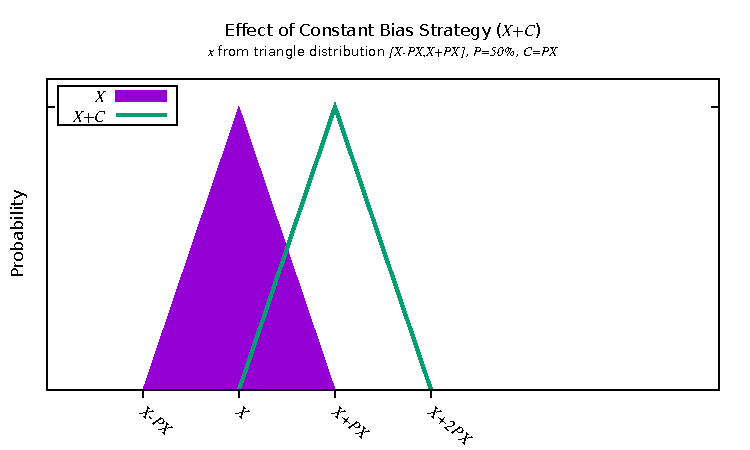
\includegraphics[width=0.5\textwidth]{figures/BiasVisualization_Constant.pdf}
		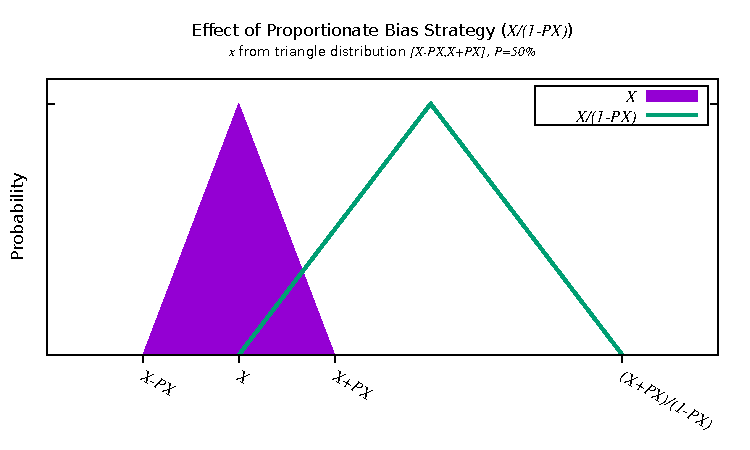
\includegraphics[width=0.5\textwidth]{figures/BiasVisualization_Proportionate.pdf}
	\end{center}
	\caption{Illustration of probabilities for a model task requirement
		with bound error as a percentage, $P$, of the actual task
		requirement, $X$, and the effect of constant and proportionate
		bias strategies transforming the distribution into
		one that never underestimates the actual term, $X$, given an
		ideal value for $C$ and $P$.  Distribution is assumed to be
		zero-mean and triangular.}
	\label{fig:cpbias}
\end{figure}

In order to achieve a less `stretched' distribution for the biased model task
requirement than the proportionate bias strategy while still maintaining the
need only for an estimated maximum percentage, not magnitude, of error, the
third proposed strategy, known as the simple bias strategy, is given in Eq.
\ref{eq:sbias}.  It fails to eliminate the possibility of underestimating
though it does reduce its propability substantially, but also prevents wildly
overestimating task requirements by decreasing the amount of `stretch' in the
biased term's distribution.  Figure \ref{fig:sbias} illustrates the effect of
the simple bias strategy on the distribution of the biased term.

\begin{equation}
\hat{X^b} \xleftarrow{s} \hat{X} (1 + P\%)
\label{eq:sbias}
\end{equation}

\begin{figure}
	\begin{center}
		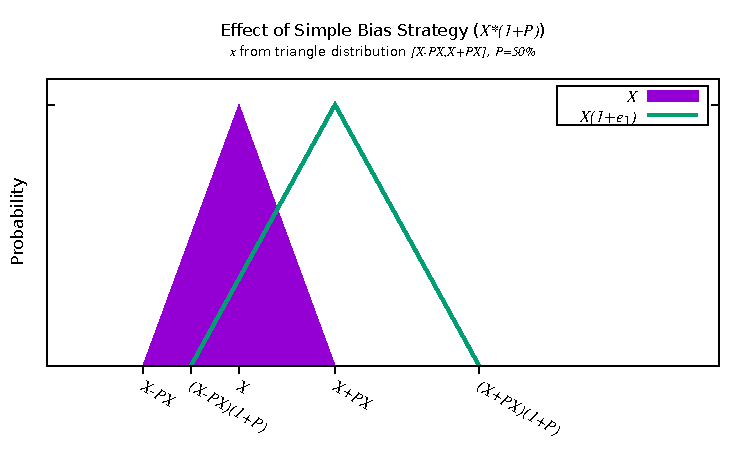
\includegraphics[width=0.5\textwidth]{figures/BiasVisualization_Simple.pdf}
	\end{center}
	\caption{Illustration of probabilities for a model task requirement
		with bound error as a percentage, $P$, of the actual task
		requirement, $X$, and the effect of the simple bias strategy
		transforming the distribution, given an ideal value for $P$.
		Distribution is assumed to be zero-mean and triangular.}
	\label{fig:cpbias}
\end{figure}

\section{Results}
\label{sec:Results}

All results were collected using simulations performed using simulator software
developed for previous research \cite{costmin} and \cite{pdpta18} and made
publically available as open source \cite{soasim}.  Workflows and task
requirements are the same as those in \cite{pdpta18} as are simulated error
amounts which ranged from $0.1\%$ up to $90\%$ taken from a uniform
distribution.  For all numeric results for performance the value presented is
an averaged value across ten simulations where the workflows and tasks were
identical but a error term applied to model tasks' requirements were unique.

\begin{figure*}
	\begin{center}
		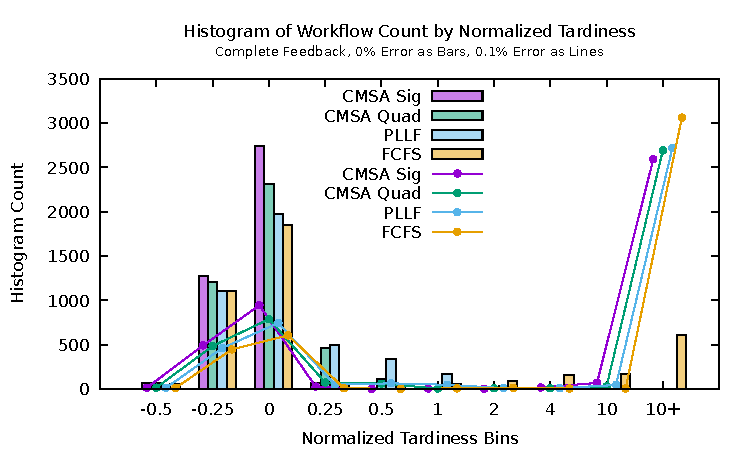
\includegraphics[width=0.9\textwidth,height=3in]{figures/Histogram_All_NoLoss_NoBias_LowError.pdf}
	\end{center}
	\caption{Histogram of workflows by normalized tardiness comparing
		relative performance of scheduling algorithms with no error (vertical
		bars) and with 0.1\% error applied to the model of the workflow
		requirements (line graphs).  Complete feedback of task completion from
		the actual platform was used, but model platform was, due to
		underestimated task requirements, allowed to model tasks as completing
		and subsequenting scheduling algorithms allowed to schedule additional
		tasks to the machine.}
	\label{fig:noloss-nobias-lowerror}
\end{figure*}

Figure \ref{fig:noloss-nobias-lowerror} shows the performance of the four
scheduling algorithms and the significant performance impact that the smallest
amount of error tested has even when complete feedback is available from the
actual platform but the model platform is still allowed to model tasks as
completing early due to underestimates of task requirements. In this figure
as with prior research, performance is depicted visually as a histogram of the
number of workflows completed in intervals based on their normalized tardiness
(the time difference between the completion and the target deadline normalized
by amount of time available to execute the workflow, i.e., the difference of
deadline and arrival time of the workflow). In this representation a normalized
tardiness of 0 represents a workflow that completed exactly at its deadline,
negative values represent workflows completed before their deadline, and
positive values those completed late.

The histogram bars of Figure \ref{fig:noloss-nobias-lowerror} represent the
performance of scheduling algorithms under the ideal circumstance of no error
in the model (i.e., the model platform perfectly predicts and represents the
resources required by a task and its execution completion time).  These
histogram bar results demonstrate how CMSA with either of the two
cost functions (Sigmoid or Quadratic) completes the largest majorities of
workflows ahead of their deadline.  The PLLF (proportional least laxity first)
algorithm completes workflows up to 4 times later (as a proportion of the
ideal finish time) than the deadline. The FCFS (first-come, first-serve)
algorithm performs relatively poorly with workflows completing far later than
their deadline because the algorithm doesn't use deadline information in making
its scheduling decisions.

The lines graphed in Figure \ref{fig:noloss-nobias-lowerror} represent the
same algorithms' histogram of workflow completion in the presence of 0.1\% error
in the model platform.  Due even to this small amount of error, the problem of
underestimating task requirements and overallocating resources, and the nature
of this issue compounding results in all four scheduling algorithms exhibiting
substantially worse performance.  This is illustrated by the reduction to less
than half as many workflow completed before their deadlines (normalized
tardinesses less than 0) compared to the no-error case.  It is also
demonstrated by the large increase of number of workflows completed with a
normalized tardiness of 10 or higher compared to the no-error case.

Therefore, with any level of partial feedback available it is unexpected that
any of these scheduling algorithms would perform better than the case of
complete feedback being available but still allowing modeling of early task
completions due to underestimated task requirements.  However, the use of
model task requirement biasing showed promising results at restoring
performance of the algorithms by eliminating or reducing the likelihood of
the underestimating problem.




\section{Summary and Future Work}
\label{sec:Summary}



\bibliography{paper}{}
\bibliographystyle{unsrt}

\end{document}

